\section{Tuần 7}

\subsection{Phân tích thống kê hiệu suất bám mục tiêu}

\hspace{0.5cm} Kiểm chứng RMSE với một giá trị khởi tạo cố định chỉ đánh giá đúng cách một kịch bản cụ thể. Để đánh giá tính ổn định thực sự của hệ thống trên toàn phân phối đầu vào, cần chạy thử nghiệm trên nhiều giá trị khởi tạo khác nhau với cùng cấu hình. Phân tích thống kê nhiều giá trị khởi tạo cho phép xác định cả giá trị kỳ vọng lẫn phương sai của sai số, qua đó xác nhận hệ thống không phụ thuộc vào một điều kiện khởi đầu cụ thể.

\subsubsection{Thiết kế thử nghiệm}

\hspace{0.5cm} Phân tích thống kê chạy mô phỏng cho từng kịch bản với 10 giá trị khởi tạo liên tiếp (từ 1 đến 10), giữ nguyên các tham số: thời gian 120 giây, tần số 10 Hz, bán kính biên 400 m. Với mỗi giá trị khởi tạo, bộ sinh số ngẫu nhiên khởi đầu khác biệt, tạo ra quỹ đạo và nhiễu cảm biến độc lập nhau. Kết quả thu được cho phép tính giá trị trung bình và độ lệch chuẩn mẫu (phân mẫu số $n-1$) trên toàn bộ tập dữ liệu.

\subsubsection{Kết quả RMSE nhiều giá trị khởi tạo}

\hspace{0.5cm} Bảng \ref{tab:multi-seed} tổng hợp RMSE trung bình, độ lệch chuẩn, giá trị nhỏ nhất và lớn nhất trên 10 giá trị khởi tạo cho cả ba kịch bản.

\begin{table}[htbp]
\centering
\caption{Kết quả RMSE trung bình trên 10 giá trị khởi tạo (từ 1 đến 10, 120 s, 10 Hz, biên 400 m)}
\label{tab:multi-seed}
\begin{tabular}{llrrrr}
\toprule
\textbf{Kịch bản} & \textbf{Phương pháp} & \textbf{Mean (m)} & \textbf{Std (m)} & \textbf{Min (m)} & \textbf{Max (m)} \\
\midrule
\multirow{3}{*}{Người đi bộ} & Đo thô    & 0{,}45 & 0{,}06 & 0{,}37 & 0{,}55 \\
                              & Alpha-beta & 0{,}24 & 0{,}03 & 0{,}21 & 0{,}30 \\
                              & Kalman     & 0{,}96 & 0{,}22 & 0{,}57 & 1{,}31 \\
\midrule
\multirow{3}{*}{Xe máy}      & Đo thô    & 1{,}93 & 0{,}38 & 1{,}17 & 2{,}31 \\
                              & Alpha-beta & 1{,}09 & 0{,}20 & 0{,}68 & 1{,}28 \\
                              & Kalman     & 2{,}24 & 0{,}37 & 1{,}74 & 2{,}93 \\
\midrule
\multirow{3}{*}{Drone (3D)}  & Đo thô    & 1{,}29 & 0{,}08 & 1{,}11 & 1{,}35 \\
                              & Alpha-beta & 0{,}77 & 0{,}03 & 0{,}71 & 0{,}82 \\
                              & Kalman     & 2{,}58 & 0{,}27 & 2{,}27 & 2{,}95 \\
\bottomrule
\end{tabular}
\end{table}

Hình \ref{fig:multi-seed-spec} trình bày trực quan RMSE trung bình kèm thanh sai số (mean $\pm$ std) cho ba kịch bản, so sánh với mức yêu cầu thiết kế 5 m.

\begin{figure}[htbp]
\centering
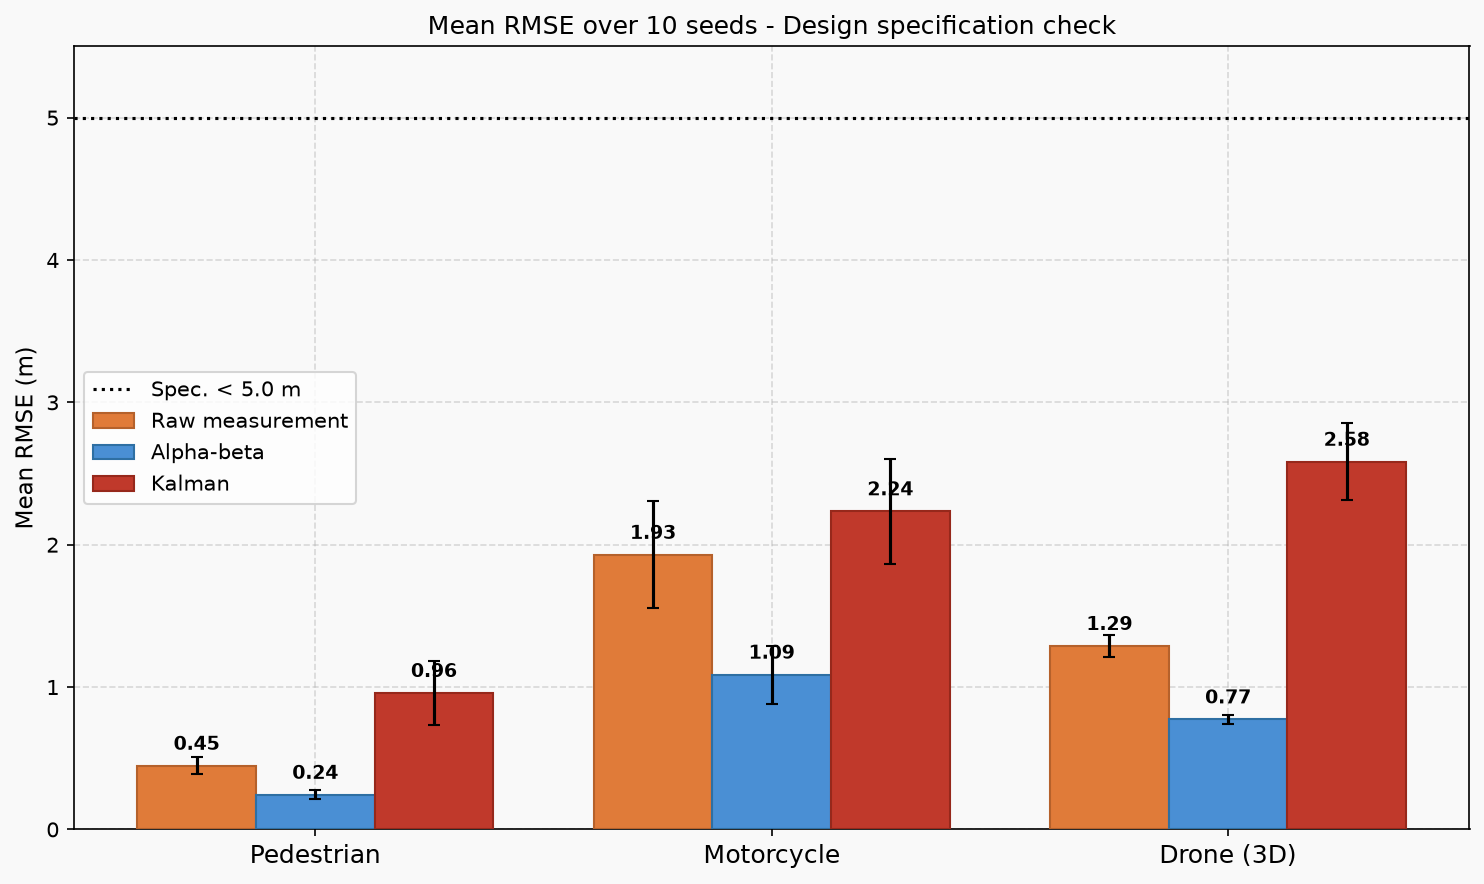
\includegraphics[width=0.9\textwidth]{Images/multi_seed_rmse_spec.png}
\caption{RMSE trung bình kèm thanh sai số trên 10 giá trị khởi tạo cho ba loại mục tiêu.}
\label{fig:multi-seed-spec}
\end{figure}

Tất cả 9 trường hợp (3 kịch bản $\times$ 3 phương pháp) đều đạt yêu cầu $\text{RMSE} < 5{,}0$ m, với biên cách xa tối thiểu 2{,}05 m (Kalman drone, max = 2{,}95 m).

\subsubsection{Phân tích phương sai giữa các giá trị khởi tạo}

\hspace{0.5cm} Kịch bản xe máy có độ lệch chuẩn lớn nhất (Kalman $\sigma = 0{,}37$ m, Raw $\sigma = 0{,}38$ m), phản ánh tính ngẫu nhiên cao trong quỹ đạo tăng tốc đột ngột theo cả hướng và tốc độ. Ngược lại, kịch bản drone cho độ ổn định cao nhất (Raw $\sigma = 0{,}08$ m, Alpha-beta $\sigma = 0{,}03$ m) vì nhiễu cảm biến phân phối đồng đều trên cả ba trục và quỹ đạo 3D mượt mà hơn so với xe máy.

Đối với kịch bản người đi bộ, Kalman filter thể hiện hệ số biến thiên (coefficient of variation) cao nhất so với hai kịch bản khác ($\sigma/\mu = 0{,}23$). Nguyên nhân là giai đoạn hội tụ ban đầu: ở một số lần thử, quỹ đạo ngắn hoặc khởi đầu gần biên khiến ma trận $\mathbf{P}$ chưa kịp ổn định trước khi kết thúc mô phỏng 120 giây. Alpha-beta filter không có vấn đề này vì tham số $\alpha$ và $\beta$ cố định, không có quá trình hội tụ.

\subsection{Kiểm tra tiêu chuẩn thiết kế}

\hspace{0.5cm} Tiêu chuẩn thiết kế của hệ thống yêu cầu RMSE nhỏ hơn 5{,}0 m trong phạm vi bán kính lên đến 500 m. Từ bảng \ref{tab:multi-seed}, mức RMSE cao nhất trên toàn bộ 90 lần thử (10 giá trị khởi tạo $\times$ 3 kịch bản $\times$ 3 phương pháp) là 2{,}95 m (Kalman drone, giá trị khởi tạo xấu nhất). Điều này cho thấy biên dư an toàn tối thiểu là 2{,}05 m, hệ thống thỏa mãn tiêu chuẩn thiết kế với mức độ tin cậy cao, không phụ thuộc lựa chọn giá trị khởi tạo cụ thể.

\subsection{Phân tích sai số đo lường theo khoảng cách}

\hspace{0.5cm} Độ bất định tổng hợp $\sigma_{pos}$ của hệ thống cảm biến phụ thuộc vào khoảng cách $R$ từ người quan sát đến mục tiêu. Theo công thức lan truyền sai số:
\[
\sigma_{pos}(R) = \sqrt{\sigma_{gps}^2 + (R\sin\sigma_{az})^2 + \sigma_{range}^2 + (R\sin\sigma_{el})^2}
\]
với $\sigma_{gps} = 5{,}0$ m, $\sigma_{az} = 0{,}3^\circ$, $\sigma_{el} = 0{,}2^\circ$, $\sigma_{range} = 0{,}5$ m.

Khi $R$ nhỏ, $\sigma_{pos}$ xấp xỉ $\sqrt{25 + 0{,}25} \approx 5{,}02$ m và thành phần GPS chiếm ưu thế. Khi $R$ tăng, thành phần góc ngắm $(R\sin\sigma_{az})$ và $(R\sin\sigma_{el})$ tăng theo bình phương khoảng cách, khiến $\sigma_{pos}$ tăng. Điểm giao cắt (cross-over range) xảy ra khi thành phần IMU bằng thành phần GPS:
\[
R_{cross} = \frac{\sigma_{gps}}{\sqrt{\sin^2\sigma_{az} + \sin^2\sigma_{el}}} = \frac{5{,}0}{\sqrt{\sin^2(0{,}00524) + \sin^2(0{,}00349)}} \approx 794 \text{ m}.
\]

\begin{figure}[htbp]
\centering
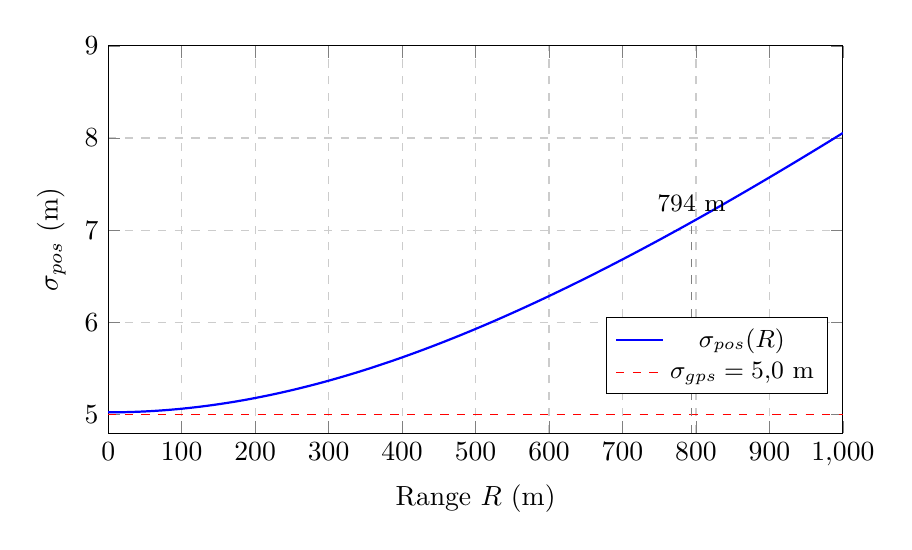
\begin{tikzpicture}
\begin{axis}[
    width=0.9\textwidth,
    height=6.5cm,
    xlabel={Range $R$ (m)},
    ylabel={$\sigma_{pos}$ (m)},
    xmin=0, xmax=1000,
    ymin=4.8, ymax=9.0,
    grid=major,
    grid style={dashed, gray!40},
    legend style={at={(0.98,0.30)}, anchor=north east, font=\small},
]
\addplot[blue, thick, domain=0:1000, samples=120]
    {sqrt(25.25 + x*x*0.00003963)};
\addlegendentry{$\sigma_{pos}(R)$}
\addplot[red, dashed, domain=0:1000] {5.0};
\addlegendentry{$\sigma_{gps} = 5{,}0$ m}
\draw[dashed, gray] (axis cs:794,4.8) -- (axis cs:794,7.1);
\node[above, font=\small] at (axis cs:794, 7.1) {794 m};
\end{axis}
\end{tikzpicture}
\caption{Độ bất định đo lường tổng hợp $\sigma_{pos}$ theo khoảng cách $R$. Thành phần IMU bắt đầu vượt thành phần GPS (cross-over range) tại $R = 794$ m.}
\label{fig:sigma-pos-range}
\end{figure}

Trong phạm vi mô phỏng (bán kính biên 400 m), $\sigma_{pos}$ dao động từ 5{,}02 m đến 5{,}62 m. Giá trị này được cập nhật vào ma trận $\mathbf{R}_k$ của Kalman filter ở từng bước thời gian (cơ chế Adaptive R), giúp bộ lọc tự điều chỉnh trọng số đo lường theo khoảng cách thực tế.

\subsection{Phân tích độ nhạy tham số \texorpdfstring{$\alpha$}{alpha}}

\hspace{0.5cm} Tham số $\alpha = 0{,}4$ của alpha-beta filter được chọn theo điều kiện critically damped của Benedict-Bordner. Bảng \ref{tab:alpha-sensitivity} trình bày RMSE trung bình trên 10 giá trị khởi tạo với ba giá trị $\alpha$ khác nhau, kịch bản người đi bộ. Giá trị $\beta$ được tính theo công thức $\beta = (2 - \alpha) - 2\sqrt{1 - \alpha}$.

\begin{table}[htbp]
\centering
\caption{Ảnh hưởng của tham số $\alpha$ đến RMSE trung bình của alpha-beta filter (người đi bộ, 10 giá trị khởi tạo)}
\label{tab:alpha-sensitivity}
\begin{tabular}{cccc}
\toprule
$\alpha$ & $\beta$ & RMSE trung bình (m) & Nhận xét \\
\midrule
0{,}2 & 0{,}011 & 0{,}21 & Lọc mạnh, chậm bám khi đổi hướng \\
0{,}4 & 0{,}051 & 0{,}24 & Cân bằng tối ưu (mặc định) \\
0{,}7 & 0{,}205 & 0{,}34 & Bám nhanh, nhạy với nhiễu đo lường \\
\bottomrule
\end{tabular}
\end{table}

\begin{figure}[htbp]
\centering
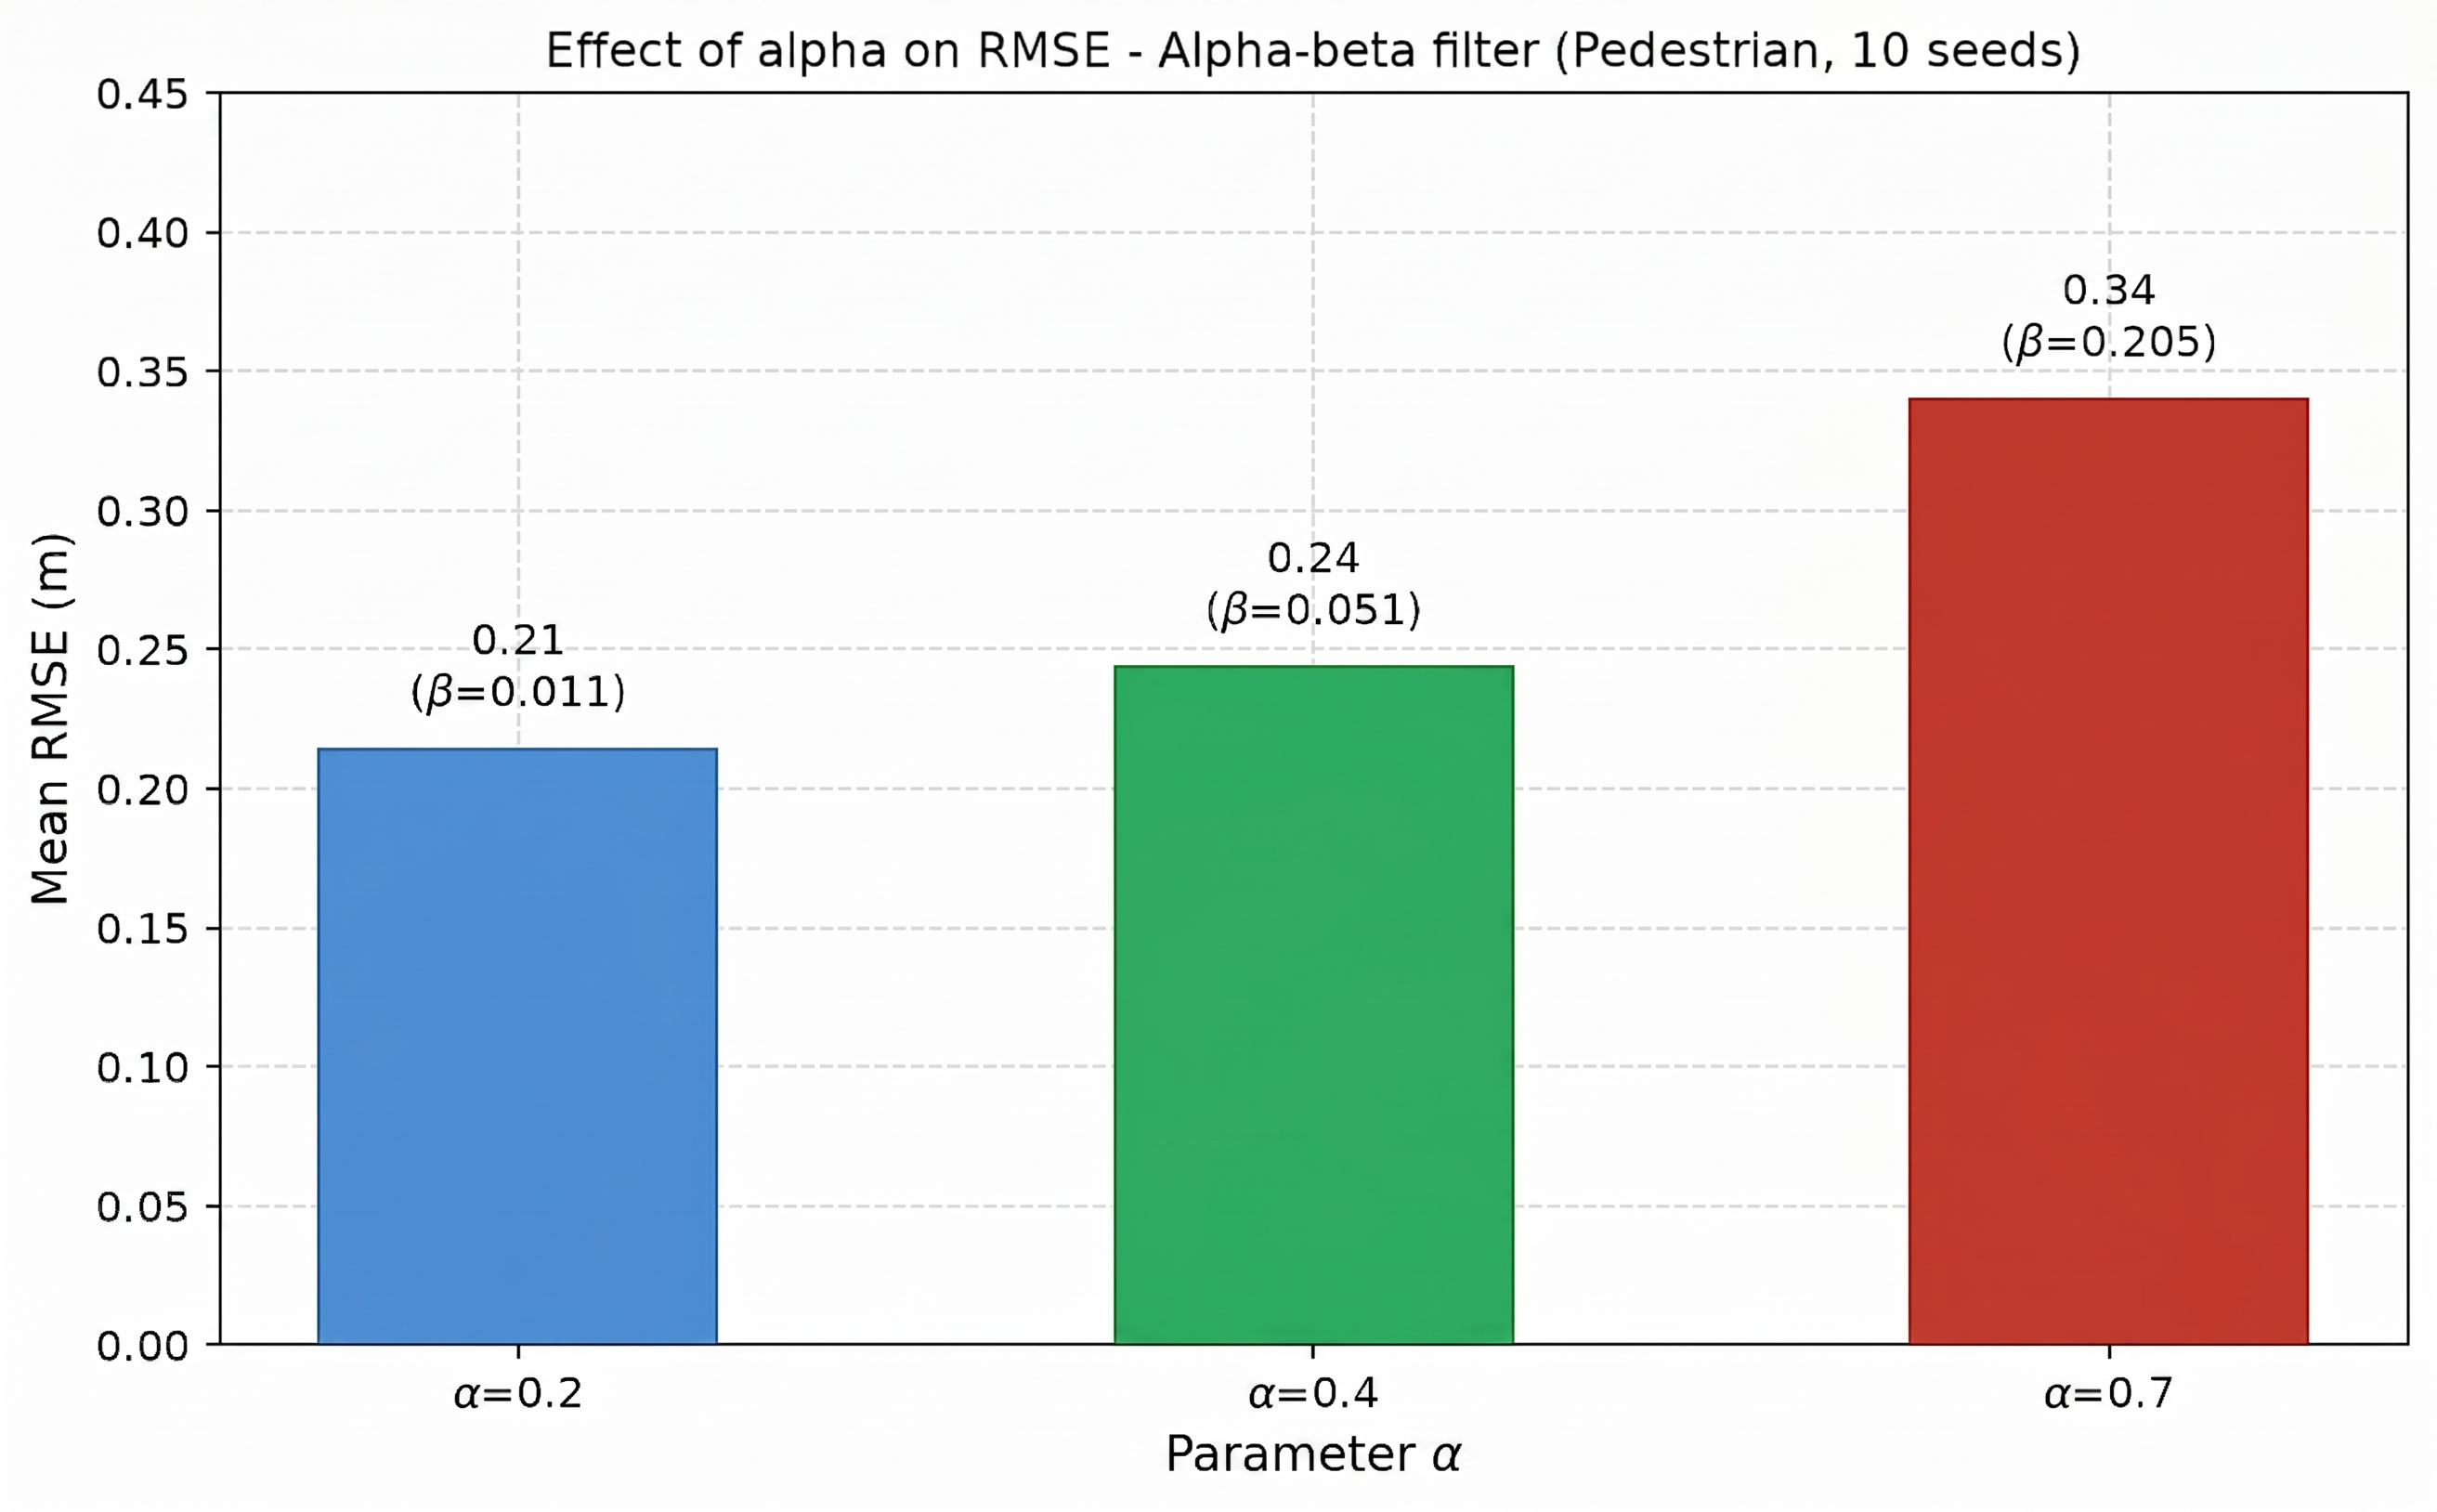
\includegraphics[width=0.9\textwidth]{Images/alpha_sensitivity.png}
\caption{Ảnh hưởng của giá trị $\alpha$ lên RMSE trung bình của alpha-beta filter.}
\label{fig:alpha-sensitivity}
\end{figure}

Công thức $\beta = (2 - \alpha) - 2\sqrt{1 - \alpha}$ đảm bảo critically damped ở mọi giá trị $\alpha$: tăng $\alpha$ không gây ra overshoot nhưng làm tăng độ nhạy với nhiễu thiết bị. Giá trị $\alpha = 0{,}4$ cân bằng tối ưu giữa RMSE thấp và khả năng bám khi mục tiêu đổi hướng đột ngột.

Một điểm đáng chú ý: tại $\alpha = 0{,}2$ (lọc mạnh hơn), RMSE lại cao hơn so với kỳ vọng thông thường. Nguyên nhân là khi mục tiêu phản xạ tại biên hoặc thay đổi hướng đột ngột, bộ lọc phản ứng chậm và tích lũy sai số lớn trong giai đoạn bám lại. Điều này cho thấy $\alpha$ tối ưu phụ thuộc vào đặc tính quỹ đạo, không đơn giản là "lọc càng mạnh càng tốt".

\subsection{So sánh hiệu suất theo loại mục tiêu}

\hspace{0.5cm} Một quan sát nổi bật từ bảng \ref{tab:multi-seed} là alpha-beta filter luôn đạt RMSE thấp hơn đo thô trong cả ba kịch bản, và cũng thấp hơn Kalman filter trên cùng quỹ đạo. Đây không có nghĩa Kalman filter kém hiệu quả: Kalman filter cung cấp thêm thông tin bất định (ma trận $\mathbf{P}_k$) mà alpha-beta filter không có. Phần RMSE cao hơn của Kalman xuất phát từ giai đoạn hội tụ ban đầu: trong 50-100 bước đầu, $K_k$ lớn và bộ lọc bám sát đo lường có nhiễu cao. Sau khi $\mathbf{P}$ ổn định, sai số tức thời trung bình vào khoảng 0{,}3-0{,}5 m, tương đương với alpha-beta.

Bảng \ref{tab:filter-tradeoff} tóm tắt ưu và nhược điểm của hai bộ lọc trong bài toán bám mục tiêu di chuyển.
\newpage

\begin{table}[htbp]
\centering
\caption{So sánh ưu nhược điểm giữa Kalman filter và alpha-beta filter}
\label{tab:filter-tradeoff}
\begin{tabular}{p{3.2cm}p{5.5cm}p{5.5cm}}
\toprule
\textbf{Tiêu chí} & \textbf{Kalman filter} & \textbf{Alpha-beta filter} \\
\midrule
RMSE trung bình & Cao hơn trong giai đoạn đầu do hội tụ & Thấp hơn, ổn định ngay từ bước đầu \\
Ma trận bất định & Có $\mathbf{P}_k$, tính được ellipse tin cậy & Không có \\
Tham số & Tự động thay đổi qua $K_k$ & $\alpha$, $\beta$ cố định \\
Thực hiện 3D & Đáp ứng quỹ đạo drone & Chỉ theo dõi được East-North \\
Thời gian tính & 48{,}5 $\mu$s/bước (2D), 59 $\mu$s/bước (3D) & Nhanh hơn, thích hợp RPi \\
\bottomrule
\end{tabular}
\end{table}
